\documentclass[11pt]{article}

\usepackage{a4wide}
\usepackage[utf8]{inputenc}
\usepackage[russian]{babel}
\usepackage{graphicx}
\usepackage{amsmath}
\usepackage{amsfonts}
\usepackage{amssymb}
\usepackage{subcaption}
\usepackage{upgreek}
\usepackage{dsfont}
\begin{document}
	
	\thispagestyle{empty}
	
	\begin{center}
		\ \vspace{-3cm}
		
		
\includegraphics[width=0.5\textwidth]{msu.eps}\\
		{\scshape Московский государственный университет имени М.~В.~Ломоносова}\\
		Факультет вычислительной математики и кибернетики\\
		Кафедра системного анализа
		
		\vfill
		
		{\LARGE Отчёт по  практикуму:}
		
		\vspace{1cm}
		
		{\Huge\bfseries <<Задача управления движением материальной точки>>}
	\end{center}
	
	\vspace{1cm}
	
	\begin{flushright}
		\large
		\textit{Студент 315 группы}\\
		А.\,В.~Бабаев
		
		\vspace{5mm}
		
		\textit{Руководитель практикума}\\
		 П.\,А.~Точилин
	\end{flushright}
	
	\vfill
	
	\begin{center}
		Москва, 2021
	\end{center}
	
	\newpage
	\tableofcontents
	\newpage
	
	{\vspace*{-2cm} \hspace*{-1cm}\section{Постановка задачи и определение параметров}}

	{\hspace{0.4cm} Движение материальной точки на прямой описывается обыкновенным дифференциальным уравнением:}
	\begin{equation}
	\ddot{x} = u_1 - \dot{x}(1 + u_2) - gx, \quad t \in [0, T] 
	\end{equation}  
	{где $x \in \mathbb{R} , u = (u_1,u_2)' \in \mathbb{R}^2$. На возможные значение управляющих параметров $u_1,u_2$ наложены следующие ограничения:}
	\begin{itemize}
		\item[1)]{либо $0 \leq u_1 \leq \alpha, u_2 \in[k_1,k_2],k_2 \geq k_1 \geq 0, $} 
		\item[2)]{либо $u_1 \in \mathbb{R}, u_2 \in [k_1,k_2], k_2 \geq k_1 \geq 0.$}
	\end{itemize}
	{Задан начальный момент времени $t_0 = 0$ и начальная позиция $x(0) : x(0) = L, \dot{x}(0) = 0.$}
	{Необходимо за счет выбора программного управления $u$ и начальной позиции перевести систему из заданной начальной позиции в такую позицию в момент времени $T$, в которой $|x(T)| + |\dot{x}(T)| \leq \upvarepsilon$. На множестве всех реализаций программных управлений, переводящих материальную точку в указанное множество, необходимо решить задачу оптимизации:}
	\begin{equation}
		J = \int_{0}^{T} u_1^2(t)dt \Rightarrow \underset{u(\cdot)}{\min}
	\end{equation}
	
	
	\begin{itemize}
		\item[1)]{Необходимо написать в среде $MatLab$ программу с пользовательским интерфейсом, которая по заданным параметрам $\alpha,T,k_1,k_2,L,\upvarepsilon$ определяет, разрешима ли задача оптимального управления (при одном из указанных двух ограничений на управления). Если задача разрешима, то программа должна построить графики компонент оптимального управления, компонент оптимальной траектории, сопряженных переменных. Кроме того, программа должна определить количество переключений найденного оптимального управления, а также моменты переключений.} 
		\item[2)]{В соответствующем заданию отчете необходимо привести все теоретические выкладки, сделанные в ходе решения задачи оптимального управления, привести примеры построенных оптимальных управлений и траекторий (с иллюстрациями). Все вспомогательные утверждения (за исключением принципа максимума Понтрягина), указанные в отчете, должны быть доказаны. В отчете должны быть приведены примеры оптимальных траекторий для всех возможных качественно различных "режимов".}
	\end{itemize}
	
	\newpage
	
	{\vspace*{-2cm} \hspace*{-1cm}\section{Теоретические выкладки}}
	{\subsection{Определение задачи и Принципа максимума Понтрягина}}
	{Запишем задачу оптимального управления:}
	\[ \ddot{x} = u_1 - \dot{x}(1 + u_2) - gx, \quad t \in [0, T],  \]
	\[ x(0) = L, \ \dot{x}(0) = 0, \]
	\[ |x(T)| + |\dot{x}(T)| = a \in [0, \upvarepsilon],  \]
	\[ \mathcal{P} =  \{ (u_1,u_2): 0 \leq u_1 \leq \alpha, u_2 \in[k_1,k_2],k_2 \geq k_1 \geq 0 \} \ \ \ \text{или} \ \ \  \mathcal{P} = \{(u_1,u_2): u_1 \in \mathbb{R}, u_2 \in [k_1,k_2], k_2 \geq k_1 \geq 0 \} \]
	\[ J = \int_{0}^{T} u_1^2(t)dt \Rightarrow \underset{u(\cdot) \in \mathcal{P}}{\min}, \]
	{где $g$ --- параметр задачи, на который в дальнейшем будут наложены некоторые ограничения. Запишем дифференциальное уравнение, описывающее закон движения, в виде системы:}
	\begin{equation}
	\begin{cases}
		\dot{x}_1 = x_2 = f_1, \\
		\dot{x}_2 = u_1 - x_2(1 + u_2) - gx_1 = f_2;
	\end{cases}
	\end{equation}
	{Итак, имеем нелинейную задачу оптимального перевода системы (3) из начальной точки $x^0 = (L,0)$ в целевое множество $\mathcal{X}(T) = \{ |x_1(T)| + |x_2(T)| \in [0, \upvarepsilon] \}$ за известное время $T$ при ограничении на допустимые управления $u \in \mathcal{P}$(в зависимости от варианта) с минимизацией функционала $J(u)$. Сформулируем принцип максимума Понтрягина для полученной задачи.}
	\newtheorem{theorem}{Теорема}
	\begin{theorem}
		{(Принцип максимума Понтрягина). Пусть $x^*(\cdot), u^*(\cdot)$ --- оптимальна пара на $[0,T],$ являющаяся решением задачи оптимального управления. Тогда существует число $\psi_0 \leq 0$ и вектор-функция $\psi(t) \in AC[0,T]$(называемая сопряженной) такие, что выполнены:}
		\begin{itemize}
			\item [1)]{условия на $\psi(t)$ \[ \dot{\psi}_i(t) = -\frac{\partial H(t,x^*(t), u^*(t),\psi(t),\psi_0)}{\partial x_i}, \quad i = 1,2 - \text{сопряженная система} \]
			\[ (\psi_0, \psi_1(t), \psi_2(t)) \neq 0 \quad \forall t \in [0,T] - \text{условие невырожденности} \]
			{где $H(t,x,u,\psi,\psi_0) = \psi_0f_0 + \langle \psi, f(t,x,u) \rangle$ --- функция Гамильтона-Понтрягина($f_0$ --- интегрант минимизируемого функционала). Для решаемой задачи:
			\[ H(t,x,u,\psi,\psi_0) = \psi_0 u_1^2 + \psi_1x_2 + \psi_2(u_1 - (1 + u_2)x_2 - gx_1); \]}	
		}
			\item [2)]{Условие максимума:
		\[ H(t,x^*(t),u^*(t),\psi(t),\psi_0) = \underset{u \in U}{\max}H(t,x^*(t),u(t),\psi(t),\psi_0) \quad \dot{\forall} t \in [0,T]; \]	
		}
			\item [3)]{Условие трансверсальности:
		\[ \psi(T) \bot \mathcal{X}(T)|_{x^*(T)}. \]	
		}
		\end{itemize}
	\end{theorem}
	{Запишем сопряженную систему из первого условия:}
	\begin{equation}
	\begin{cases}
	\dot{\psi_1} = g\psi_2,	\\
	\dot{\psi_2} = -\psi_1 + \psi_2(1 + u_2);
	\end{cases}
	\end{equation}	
	{Так как полученная система однородна, $\psi(t)$ определяется с точностью до умножения на константу. Также домножение ($\psi_0,\psi_1(t),\psi_2(t)$) на положительную константу не нарушит условия максимума.}
	
	
	{\subsection{Вычисление оптимального управления}}
	{Найдем оптимальное управление $u^* = (u_1^*, u_2^*)$ из условия максимума, т.е. оно должно максимизировать функцию Гамильтона-Понтрягина $H$:}
	\[ H(t,x,u,\psi,\psi_0) = \psi_0 u_1^2 + \psi_1x_2 + \psi_2(u_1 - (1 + u_2)x_2 - gx_1). \]
	{Рассмотрим первую компоненту $u_1^*$:}
	\[ \psi_0u_1^2 + \psi_2 u_1 \Rightarrow \underset{u_1}{\max}, \]
	{Ограничение на компоненту управления $u_1^*$ в первом варианте: $0 \leq u_1 \leq \alpha$}
	\begin{itemize}
		\item [1.]{при $\psi_0 \neq 0 $ 
		\[ u_1^* = \begin{cases}
		-\frac{\psi_2}{2\psi_0}, & 0 < -\frac{\psi_2}{2\psi_0} < \alpha, \\
		0,& -\frac{\psi_2}{2\psi_0} < 0,\\
		\alpha,& -\frac{\psi_2}{2\psi_0} > \alpha;
		\end{cases} \]	
	}
		\item [2.]{при $\psi_0 = 0 $
	\[ u_1^* = \begin{cases}
	0,& \psi_2 < 0,\\
	\alpha,& \psi_2 > 0,\\
	[0, \alpha],& \psi_2 = 0;
	\end{cases} \]		}
	\end{itemize}
	{Ограничение на компоненту управления $u_1^*$ во втором варианте: $u_1 \in \mathbb{R}$}
	\begin{itemize}
		\item [1.]{при $\psi_0 \neq 0 $ 
			\[ u_1^* = -\frac{\psi_2}{2\psi_0} ,\]
		}
		\item [2.]{при $\psi_0 = 0 $
			\[ u_1^* = \pm \infty, \quad \text{т.е. задача оптимизации не разрешима.} \]	}
	\end{itemize}
	{Рассмотрим вторую компоненту $u_2^*:$}
	\[-\psi_2u_2x_2 \Rightarrow \underset{u_2}{\max}. \]
	{Ограничение на компоненту управления $u_2^*$ в обоих вариантах: $u_2 \in [k_1,k_2], k_2 \geq k_1 \geq 0,$ максимизируемое выражение не зависит от $\psi_0.$}
	\[ u_2^* = \begin{cases}
	k_1,&  \psi_2x_2 > 0,\\
	k_2,& \psi_2x_2 < 0,\\
	[k_1,k_2],&  \psi_2x_2 = 0;
	\end{cases} \]
	
	\subsection{Формула Коши для $x(t)$ и $\psi(t)$}
	\begin{theorem}
		{(Формула Коши). Решение задачи Коши для неоднородной линейной системы обыкновенных дифференциальных уравнений:}
		\[ \begin{cases}
			\frac{dy}{dt} = Ay(t) + f(t),\\
			y(t_0) = y^0;
		\end{cases} \]
		{представимо в виде:}
		\[y(t) = W(t,t_0)y^0 + \int_{t_0}^{t} W(t,\tau) f(\tau)d\tau, \]
		{где $W(t,\tau) = e^{A(t - \tau)}$ --- фундаментальная матрица системы.}
	\end{theorem}
	{Введем следующие обозначения:}
	\[ A_x^{u_2}  = \left( \begin{matrix}
	0 & 1 \\
	-g & -(1 + u_2)
	\end{matrix} \right), f^{u_1} = \begin{pmatrix}
	0\\
	u_1
	\end{pmatrix}, x^0 = \begin{pmatrix}
	x_1^0\\
	x_2^0
	\end{pmatrix},  \]
	\[ A_\psi^{u_2} = \begin{pmatrix}
	0 & g \\
	-1 & 1 + u_2
	\end{pmatrix}, \psi^0 = \begin{pmatrix}
	\psi_1^0 \\
	\psi_2^0
	\end{pmatrix} \]
	{Система (3) примет вид:}
	\[ \begin{cases}
	\dot{x} = A_x^{u_2}x + f^{u_1}, \\
	x(t_0) = x^0.
	\end{cases} \]
	{По формуле Коши решение системы (3) для промежутков времени, на которых компонента управления $u_2$ постоянна, имеет вид:}
	\begin{equation}
	x(t) = e^{A_x^{u_2}(t - t_0)}x^0 + \int_{t_0}^{t}\exp\{A_x^{u_2}(t - \tau)\}f^{u_1}(\tau)d\tau.
	\end{equation}
	{Сопряженная система (4) примет вид:}
	\[ \begin{cases}
	\dot{\psi} = A_\psi^{u_2}\psi,\\
	\psi(t_0) = \psi^0.
	\end{cases} \]
	{По формуле Коши решение сопряженной системы (4) для промежутков времени, на которых компонента времени $u_2$ постоянна, имеет вид:}
	\begin{equation}
	\psi(t) = e^{A_\psi^{u_2}(t - t_0)}\psi^0.
	\end{equation}
	
	
	\subsection{Об особых режимах}
	{При $\psi_2x_2 =0$ возможен особый режим, в этом случае компонента управления $u_2$ восстанавливается неоднозначно. Рассмотрим условия возникновения особого режима.}
	\begin{itemize}
		\item [1.]{Если $x_2(t^{'})= 0$
	\newline
	Покажем, что при этом условии нет особого режима. При $x_2 = 0$ компонента управления $u_2$ не влияет на траекторию системы, поэтому $u_2$ можно взять любым.	
	}
		\item [2.]{Если $\psi_2(t^{'}) = 0$
	\newline
	Возникает возможность особого режима, т.е невозможность однозначно определить компоненту управления $u_2 \in [k_1,k_2].$ Но если система находится в этом режиме, то она стоит в нуле, и если сразу не выйти из него, то получится тривиальный случай задачи.	
	}
	\end{itemize}

	\subsection{О перепараметризации}
	{Для решения задачи необходимо построить все траектории, получающиеся при управлениях из принципа максимума, из них выбрать, те которые попадают в целевое множество $\mathcal{X}(T)$ в финальный момент времени $T$, и из полученных выбрать оптимальную пару, которая минимизирует функционал.
	\newline
	 Из получившегося по принципу максимума вида оптимального управления, следует что переключения управления $u^*$ возможны при $\psi_2(t) = 0, x_2(t) = 0$ в обоих вариантах (вид компоненты $u_2^*$ для них общий), а также при $\psi_2 = \alpha$ в случае $\psi_0 < 0$ первого варианта. В предыдущем разделе было показано, что эти переключения простые, т.е. в задаче не возникает особых режимов.
	 \newline
	 Для того чтобы найти время первого переключения управления $u^*$ необходимо получить зависимости $x(t),  \psi(t)$, проинтегрировав систему на $x(t)$ и сопряженную систему, что невозможно без знания начальных значений $\psi_1^1,\psi_2^0$. Если знать эти начальные значения, то решив задачу Коши для $x(t),\psi(t) $ из начальной позиции $(L,0,\psi_1^0,\psi_2^0),$ можно найти время первого переключения $t^*$ и получить связь между $(\psi_1^0,\psi_2^0)$ и $t^*$. Далее изменив систему на $x(t)$ и сопряженную систему(смена управления), имеем задачу Коши с начальной позицией($x_1(t^*),x_2(t^*),\psi_1(t^*),\psi_2(t^*)$) для дальнейшего получения $x(t), \psi(t)$.
	 \newline
	 Но $\psi_1^0$ и $\psi_2^0$	не даны. Перебор по ним невозможен в силу неограниченности множества ($\psi_1^0,\psi_2^0 \in \mathbb{R}$, поскольку нет никаких данных по начальным условиям сопряженной системы) их значений. Поэтому обратим задачу: будем искать ($\psi_1^0,\psi_2^0$) из их связи с временем первого переключения $t^*$, перебирая по возможным значениям $t^*$. А это уже перебор по конечному множеству. Если не удастся поточнее оценить $t^*$, то можно перебирать его по всему временному отрезку $[0, T]$, так как финальное время $T$ не очень велико.
	 \newline
	 Уточним, для перепараметризации задачи недостаточно одного времени первого переключения $t^*$, но его связь с нужными ($\psi_1^0,\psi_2^0$) дает возможность перебора по $t^*$, что вместе с еще одним конечным перебором по какому-либо параметру позволит заменить неограниченный перебор на конечный. Вторым параметром в зависимости от случая может быть $\psi_1$ или $\psi_2$, если они приемлемо ограничены (в первом варианте задачи таким параметром будет являться $\psi_2$ поскольку он принадлежит сегменту $[0,\alpha]$ по условию и как раз для решения задачи, я делал перебор по данному элементу, а на $\psi_1$ не было ограничений, и поэтому он не считается приемлемо ограниченным), или время второго переключения $t^{**}$.
	 
	 
	 \section{Исследование задачи в первом варианте}
	 {Ограничения на допустимые управления имеют вид:}
	 \[ u \in \mathcal{P} = \{(u_1,u_2): 0 \leq u_1 \leq \alpha, u_2 \in[k_1,k_2],k_2 \geq k_1 \geq 0 \} \]
	 
	 \subsection{Нормальный случай: $\psi_0 < 0$}
	 {Пусть $\psi_0 = -\frac{1}{2}$, т.к. ($\psi_0,\psi(t)$) определяются с точностью до умножения на положительную константу. Тогда компоненты оптимального управления имеют вид:}
	 \begin{equation}
	 u_1^* = \begin{cases}
	 0, & \psi_2 < 0, \\
	 \psi_2, & 0 < \psi_2 < \alpha,\\
	 \alpha, & \psi_2 > \alpha;
	 \end{cases}
	 \end{equation}
	 \begin{equation}
	 u_2^* = \begin{cases}
	 k_1, & \psi_2x_2 > 0, \\
	 k_2, & 0 < \psi_2x_2 < 0,\\
	 [k_1,k_2], & \psi_2x_2 = 0;
	 \end{cases}
	 \end{equation}
	 
	 \subsubsection{Случай $\psi_2^0 > 0$}
	 {Рассмотрим поведение системы в окрестности начального времени $t_0 = 0.$ Так как $\psi_2^0 > 0,$ то компонента управления $u_1^*$ может принимать следующие значения:}
	 \[ u_1^* = \begin{cases}
	 \psi_2, \ 0 < \psi_2 < \alpha\\
	 \alpha, \ \psi_2 > \alpha
	 \end{cases} \Rightarrow u_1 > 0 \ \text{в окрестности }  t_0 = 0,\]
	 \[ \dot{x}_2(0) = [u_1 - x_2(1 + u_2)-gx_1]|_{t = 0} = \{x^0 = (L,0) \} = u_1(0) - gL. \]
	 {В силу произвольности вводимых данных, значение данного выражения может быть любым, поэтому будем считать что оно положительно (для отрицательного случая все рассуждения аналогичны), а случай равенства нулю будет разобран позже.}
	 \newline
	 {Из положительности следует, что $x_2(t)$ возрастает в окрестности $t_0 = 0$, следовательно, $x_2(t) > 0$ т.к. $x_2(0) = 0.$ Так как $\psi_2^0 > 0$ и система рассматривается до первого переключения по $\psi_2(t^*) = 0,$ то $ \psi_2(t) > 0$ до времени $t^*$. Из этого вытекает, что $\psi_2x_2 > 0$ в окрестности $t_0 = 0.$ }
	 \newline
	 {До переключения по $\psi_2(t^*) = 0$ возможно переключение $\psi_2(t_{\alpha}) = \alpha.$ Но при нем изменится компонента $u_1^*$, что не повлияет на сопряженную систему. Проблема возникает с доказательством отсутствия переключения $x_2(t) = 0.$ Получено, что $x_2(t) > 0$ и компонента управления $u_2^* = k_1$ в окрестности $t_0 = 0.$ Доказательство того, что $x_2(t) > 0$ и дальше до переключения по $\psi_2(t^*) = 0$, приводится далее при рассмотрении всех возможностей поведения $\psi_2(t)$.}
	 \newline
	 {Итак, в этом случае система решается при компоненте управления $u_2^* = k_1$ до времени первого переключения по $\psi_2(t^*) = 0.$ Поэтому по формуле (6) при фиксированных $\psi_1^0,\psi_2^0$ получим:}
	 \begin{equation}
	   \psi(t) = e^{A^{k_1}_\psi t}\psi^0 \Rightarrow \psi_2(t) = \frac{e^{\frac{t}{2}(1 + k_1)}}{p}[(-2\psi_1^0 + (1+k_1)\psi_2^0)\sinh\frac{p}{2}t + p\psi_2^0\cosh\frac{p}{2}t], 
	 \end{equation}
	 {где $p = \sqrt{k_1^2 + 2k_1 -4g + 1}.$ Получим ограничения на возможные входные параметры задачи:}
	 \begin{equation}
	 k_1^2 + 2k_1 -4g + 1 > 0.
	 \end{equation}
	 {Получим связь параметров $\psi_1^0,\psi_2^0$ и временем первого переключения $t^*$ из условия
	\newline 	
	 	 $\psi_2(t^*) = 0:$}
	 \begin{equation}
	 \tanh\frac{p}{2}t^* = \frac{p\psi_2^0}{2\psi_1^0 - (1 + k_1)\psi_2^0}.
	 \end{equation}
	 {Область значений гиперболического тангенса при положительном аргументе: (0,1), поэтому:}
	 \begin{itemize}
	 	\item [1.]{$\psi_2(t)$ не пересекает ноль, если:
		\[ \frac{p\psi_2^0}{2\psi_1^0 - (1 + k_1)\psi_2^0} \leq 0 \ \text{  или  }\ \frac{p\psi_2^0}{2\psi_1^0 - (1 + k_1)\psi_2^0} \geq 0. \]
		Cледовательно  $\psi_1^0 \leq \frac{\psi_2^0}{2}(1 + k_1).$ В этом случае функция $\psi_2(t)$ возрастает. 	
 	}
	 	\item [2.]{$\psi_2(t)$ пересекает ноль, если:
		\[0 < \frac{p\psi_2^0}{2\psi_1^0 - (1 + k_1)\psi_2^0} < 1 \Rightarrow \psi_1^0 > \frac{\psi_2^0}{1}(p + (1 + k_1)). \]
		Возможны два варианта поведения функции $\psi_2(t)$ до пересечения с нулем: монотонно убывает или сначала колеблется а потом убывает.	 	
 }
	 \end{itemize}
 	{Формула (9) и последующие рассуждения о поведении системы в каждом случае, приводятся в предположении о необнулении функции $x_2(t)$ до времени первого переключения по $\psi_2(t^*)= 0,$ а, следовательно, в предположении о том, что система до времени $t^*$ решается при компоненте управления $u_2^* = k_1$. }
 	\newline
 	{\textbf{Первый случай: $\psi_2(t)$ не пересекает ноль}}
 	\newline
 	{Во-первых, необходимо доказать, что $x_2$ при таком поведении $\psi_2(t)$ не обнуляется до переключения по $\psi_2(t^*) = 0.$ Во-вторых, необходимо получить нужную перепараметризацию. Так как поведение всей системы зависит от компоненты $u_1^*$ и возможны два ее значения до переключения по $\psi_2(t^*) = 0,$ рассмотрим следующие два случая: $\psi_2^0 \geq \alpha$ или $\psi_2^0 < \alpha.$ }
 	
 	\begin{itemize}
 		\item [(a)]{$\psi_2^0\geq \alpha$ (случай без переключений)
 		\newline
 		По формуле (7) для компоненты управления $u_1^*$ получим ее начальное значение $u_1^*= \alpha$. Переключение по $\psi_2(t_{\alpha} = \alpha)$ невозможно в силу возрастания функции $\psi_2(t)$ из начального значения $\psi_2^0 \geq \alpha$
 		\newline
 		Рассмотрим знак функции $x_2(t):$
 		\begin{equation}
 		x(t) = \int_{t_0}^{t}\exp\{A_x^{k_1}(t - \tau)\}\begin{pmatrix}
 		0\\
 		\alpha
 		\end{pmatrix}d\tau
 		\Rightarrow x_2(t) = \frac{2\alpha e^{-\frac{t}{2}(1 + k_1)}}{p}\sinh\frac{p}{2}t > 0.
 		\end{equation}
 		Итак, в этом случае переключения управления нет. Поэтому перепараметризация не нужна, т.к. решение сопряженной системы не требуется для интегрирования системы (3). Решив систему на $x(t)$ при управлении $u_1^* = \alpha,u_2^* = k_1$ из начальной точки $x^0 = (L,0)$ до финального времени $T$, проверяем попадание траектории в целевое множество $\mathcal{X}(T).$ Если $x(T)\in \mathcal{X}(T), $ то полученная пара $(x(t),u^*(t))$ подлежит дальнейшему рассмотрению на минимизацию функционала. 	
 	}
 		\item [(b)]{$\psi_2^0 < \alpha$
 		\newline
 		По формуле (7) для компоненты $u_1^*$ получим, что система стартует с $u_1^* = \psi_2(t).$ Так как $\psi_2^0$ и функция $\psi_2(t)$ возрастает, получим при $\psi_2(t_{\alpha}) = \alpha$ компонента управления $u_1^*$ переключается с $\psi_2(t)$ на $\alpha.$ Введем новый параметр --- время этого переключения $t_{\alpha}.$ Как уже пояснялось, это переключение не повлияет на сопряженную систему, поэтому по формуле (9) из условия $\psi_2(t_{\alpha}) = \alpha$ получим связь ($\psi_1^0,\psi_2^0$) и параметра $t_{\alpha}:$
 		\begin{equation}
 		\psi_1^0 = \frac{1}{2\sinh\frac{p}{2}t_{\alpha}}[((1 + k_1)\sinh\frac{p}{2}t_{\alpha} + p\cosh\frac{p}{2}t_{\alpha})\psi_2^0 - \alpha pe^{-\frac{t_{\alpha}}{2}(1 + k_1)}].
 		\end{equation} 
 	}
 	\end{itemize}
 	Осталось показать, что функция $x_2(t)$ не обращается в нуль до времени $t_{\alpha}$. Предполагалось доказательство до $t^*$, но это лишнее, т.к. задача Коши для системы после первого интегрирования задана и подлежит численному интегрированию. По формуле (5) получим:
 	\[ x(t) = \int_{t_0}^{t}\exp\{A_x^{k_1}(t - \tau)\}\begin{pmatrix}
 	0\\
 	\psi_2(\tau)
 	\end{pmatrix}d\tau, \]
 	где $\psi_2(\tau)$ определяется формулой (9). Для второй компоненты получим:
 	\begin{equation}
 	x_2(t) = \frac{e^{-\frac{t}{2}(1 + k_1)}}{2(1+k_1)p}[(e^{t(1 + k_1)} - 1)p\psi_2^0\cosh\frac{p}{2}t - [2(e^{t(1 + k_1)} - 1)\psi_1^0 - (1 + k_1)(e^{t(1 + k_1)}+1)\psi_2^0]\sinh\frac{p}{2}t].
 	\end{equation} 
 	Использую ограничение этого случая на $\psi_1^0,\psi_2^0: -2\psi_1^0 > -(p + (1 + k_1))\psi_2^0$ оценим полученное выражение для $x_2(t):$
 	\newcommand{\sgn}{\text{sgn}}
 	\[ -[2(e^{t(1 + k_1)} - 1)\psi_1^0 - (1 + k_1)(e^{t(1 + k_1)} + 1)\psi_2^0] > [p(1 - e^{t(1 + k_1)}) + 2(1 + k_1)]\psi_2^0 \Rightarrow \sgn[x_2(t)] > 0.\]
 	\textbf{Итак, получена перепараметризация $\psi_2^0 \in [0,\alpha], t_{\alpha} \in [0, T]$ и формула связи (13).}
 	\newline
 	\newline
 	\textbf{Второй случай: $\psi_2(t)$ пересекает ноль}
 	\newline
 	{Как было показано, этот случай возможен при $\psi_1^0 > \frac{\psi_2^0}{2}(p + (1 + k_1)).$ Функция $\psi_2(t)$ до пересечение с нулем может: либо монотонно убывать, либо до окрестности нуля как-то произвольно вести себя, а в окрестности убывать. Но цель этого пункта получить корректную перепараметризацию задачи, а для этого нужно исследовать поведение системы до первого, если надо второго, переключения. Рассмотрим три возможных случая начального значения $\psi_2^0$ и поведения функции $\psi_2(t)$.}
 	\begin{itemize}
 		\item [(a)]{$\psi_2^0 > \alpha .$
 		\newline
 		До переключения $\psi_2(t_\alpha)=\alpha$ система решается с $u_1^* = \alpha,u_2^*=k_1$. Поэтому функция $x_2(t)$ положительна до переключения $t_\alpha$ по формуле (12). По формуле (9) из условия $\psi_2(t_\alpha) = \alpha$ получим связь параметров $(\psi_1^0,\psi_2^0)$ и времени первого переключения $t_\alpha$, которая выражается формулой (13):
 		\[ \psi_1^0 = \frac{1}{2\sinh\frac{p}{2}t_{\alpha}}[((1 + k_1)\sinh\frac{p}{2}t_{\alpha} + p\cosh\frac{p}{2}t_{\alpha})\psi_2^0 - \alpha pe^{-\frac{t_{\alpha}}{2}(1 + k_1)}]. \]
 		Так как $\{\psi_2 > \alpha\}$ - неограниченное множество, нужен еще один параметр: время переключения по $\psi_2(t^*) = 0.$ После переключения по $\psi_2(t_\alpha) = \alpha$ компонента управления $u_1^*$ изменится с $\alpha$ на $\psi_2$ а вторая компонента останется прежней $u_2^* = k_1.$ Рассмотрим пересечение функции $\psi_2(t)$ с нулем, оно описывается формулой (11). Подставим в нее полученную в формуле (13) связь $\psi_1^0$ с $\psi_2^0,t_\alpha.$ Получим связь $\psi_2^0$ от новых параметров $t_\alpha,t^*:$
 		\begin{equation}
 		\psi_2^0 = \alpha e^{-\frac{t_\alpha}{2}(1 + k_1)} \frac{\sinh\frac{p}{2}t^*}{\sinh \frac{p}{2}(t^* - t_\alpha)}.
 		\end{equation}
 		Осталось проверить, что функция $x_2(t)$ положительна при $0 < \psi_2(t) < \alpha.$ Поведение $x_2(t)$ при $t \in [t_\alpha, t^*]$ описывается формулой второй компоненты функции:
 		\[ x(t) = e^{A_x^{k_1}(t - t_\alpha)}x(t_\alpha) + \int_{t\alpha}^{t}\exp\{A_x^{k_1}(t - \tau) \}\begin{pmatrix}
 		0\\
 		\psi_2(\tau)
 		\end{pmatrix}d\tau, \]
 		где $x(t_\alpha)$ определяется формулой (12), а $\psi_2(\tau)$ формулой (9). Из-за громоздкости  выражений не будем приводить доказательство положительности $x_2(t)$. Оно проводится аналогично предыдущему.
 		\newline
 		\textbf{Итак, получена перепараметризация $0 < t_\alpha < t^* \leq T $ и формулы связи (13), (15).}
  	}
 		\item [(b)]{$\psi_2^0 \leq \alpha$ и $\psi_2(t)$ всегда меньше $\alpha.$
 		\newline	
 		До переключения по $\psi_2(t^*) = 0$ система решается при $u_1^* = \psi_2,u_2^* = k_1.$ Так как функция $\psi_2(t)$ не зависит от компоненты $u_1^*$, то из формулы (11) получим связь $\psi_1^0$ с $\psi_2^0,t^*$:
 		\begin{equation}
 		\psi_1^0 = \frac{1}{2}\psi_2^0[p\coth\frac{p}{2}t^* + 1 + k_1].
 		\end{equation}
 		Доказательство положительности функции $x_2(t)$ до переключения $\psi_2(t^*) = 0$ аналогично подслучаю (b) первого случая.
 		\newline
 		\textbf{Итак, получена перепараметризация: $\psi_2^0 \in (0, \alpha], t^* \in [0,T]$ и формула связи (16).}
 	}
 	\item[(c)]{$\psi_2^0 \leq \alpha$ и  $\psi_2(t)$ пересекает $\alpha.$
 	\newline
 	В этом случае функция $\psi_2(t)$ не сразу убывает у нулю. До переключения $\psi_2(t_\alpha) = \alpha$ система решается при $u_1^* = \psi_2, u_2^* = k_1.$ Так функция $\psi_2(t)$ не зависит от компоненты $u_1^*$, то из формулы (13) получим связь $\psi_1^0$ c $\psi_2^0,t_\alpha:$	
 	\[\psi_1^0 = \frac{1}{2\sinh\frac{p}{2}t_{\alpha}}[((1 + k_1)\sinh\frac{p}{2}t_{\alpha} + p\cosh\frac{p}{2}t_{\alpha})\psi_2^0 - \alpha pe^{-\frac{t_{\alpha}}{2}(1 + k_1)}].\]
 	Доказательство положительности функции $x_2(t)$ до переключения $\psi_2(t_\alpha) = \alpha$ аналогично подслучаю (b) первого случая. 
 	\newline 
 	\textbf{Итак, получена перепараметризация: $\psi_2^0 \in (0,\alpha],t_\alpha \in [0, T]$ и формула связи (13).}
 }
 	\end{itemize}
 
 \subsubsection{Случай $\psi_2^0 \leq 0$}
 {Пусть $\psi_2^0 < 0.$ Тогда по формуле (7): $u_1^*|_{t = 0} = 0$. Следовательно:}
 \begin{equation}
 \dot{x}_2(0) = [u_1 - x_2(1 + u_2) - gx_1]|_{t = 0} = -gL.
 \end{equation}
 {Данный случай, когда правая часть ненулевая аналогичен предыдущему рассмотренному. Поэтому логично предположить, что правая часть ноль, $(gL = 0)$ чтобы рассмотреть все случаи. $x_2 = const = x_2(0) = 0$ в окрестности $t = 0,$ причем достаточно большой окрестности: пока $u_1 = 0 \Rightarrow u_2^*$ не определена в этой окрестности $t = 0,$ но компонента $u_2$ не влияет на равенство (17), поэтому можно взять любое значение из возможных $[k_1,k_2],$ пусть $u_2 = k_1$. Итак, особый режим предотвращается, т.к. удается однозначно задать компоненту управления $u_2(t)$ в то время пока система стоит в нуле.
\newline
Вывести систему из этого состояния может только компонента управления $u_1:$ когда она станет ненулевой(пусть $t^{'}-$ время, когда она перестанет быть нулем) получим: 
\[ \dot{x}_2(t^{'}) = [u_1 - x_2(1 + k_1) - gx_1]|_{t = t^{'}} = u_1(t^{'}) > 0. \]
Следовательно, функция $x_2(t)$ начнет расти из нуля и система стронется с места, а вторая компонента управления останется прежней $u_2 = k_1$ по крайней мере в окрестности $t = t^{'}$, т.к. $\psi_2 x_2 >0$ в этой окрестности. Этот факт нужен для дальнейших рассуждений о неотрицательности $x_2(t)$ между переключениями по $\psi_2(t)$.
\newline
Компонента $u_1(T)$ перестанет быть нулевой за счет переключения по $\psi_2(t^{'}) = 0.$ Ведь в то время пока система стоит, сопряженные функции меняются. Подробнее, функция $\psi_2(t)$ должна возрастать.
\newline
Запишем уравнение сопряженной системы $\dot{\psi}_2 = - \psi_1 + \psi_2(1 + k_1) $ до времени $t^{'}$. Начальное значение $\psi_1^0 < 0$, т.к. иначе получим: $\dot{\psi}_2(0) = -\psi_1^0 + \psi_2^0(1 + k_1) < 0 \Rightarrow\psi_2(t)$ убывает от $\psi_2^0 < 0\Rightarrow \psi_2(t)$ не пересечет ноль, и компонента $u_1$ не станет положительной, и система останется в нуле.
\newline
Пока $-\psi_1 < \psi_2(1 + k_1)$ получим, что  $\dot{\psi_2} < 0 \Rightarrow \psi_2(t)$ убывает из начального значения $\psi_2^0 < 0 \Rightarrow \psi_2(t) < 0 \Rightarrow \dot{\psi}_1 = \psi_2 < 0 \Rightarrow \psi_1(t)$ убывает из начального значения $\psi_1^0 < 0 \Rightarrow$ наступит момент, когда $-\psi_1 > \psi_2 (1 + k_1)\Rightarrow \dot{\psi}_2 > 0 \Rightarrow \psi_2(t)$ начнет возрастать.
\newline
Итак, в момент времени $t^{'}:\psi_2(t^{'}) = 0$ происходит переключение компоненты $u_1^*$ на положительное $\psi_2.$ Система выходит из нуля. Если $\psi_2^0 = 0,$ то система сразу выходит из нуля, $t^{'} = 0.$
\newline
Введем новый параметр: $t^{'}$. До выхода из нуля решение сопряженной системы для $\psi_2(t)$ имеет вид (9), поэтому связь между $(\psi_1^0,\psi_2^0)$ и $t^{'}$ выражается формулой (11). Пересечение функции $\psi_2(t)$ с нулем будет, т.к. доказано, что $\psi_2(t)$ возрастает из начального значения $\psi_2^0$.
\newline
Далее система ведет себя следующим образом: поведение функции $\psi_2(t)$ не изменится, т.к. переключение компоненты $u_1^*$ не влияет на сопряженную систему, поэтому она продолжает возрастать до пересечения с $\alpha$. Введем необходимый второй параметр $t_\alpha:\psi(t_\alpha) = \alpha.$ Формулой связи между $(\psi_1^0,\psi_2^0)$ и $t^{'}$ является формула (13).
\newline
Аналогично случаю 3.1.1 в этом режиме доказывается, что переключений по $x_2(t) = 0$ не будет, эта функция останется положительной. Вспомогательный для этого факт неотрицательности в окрестности $t^{'}$ доказан.
\newline
\textbf{Итак, получена перепараметризация: $0 < t^{'} < t_\alpha \leq T$ и формулы связи (11) и (13).}
}
\subsection{Анормальный случай: $\psi_0 = 0.$}
{Из принципа максимума получено, что компоненты оптимального управления имеют вид:
\begin{equation}
u_1^* = \begin{cases}
0, & \psi_2 > 0,\\
\alpha, & \psi_2 < 0,\\
[0,\alpha], & \psi_2 = 0;
\end{cases}
\end{equation}

\begin{equation}
u_2^* = \begin{cases}
k_1, & \psi_2x_2 > 0,\\
k_2, & \psi_2x_2 < 0,\\
[k_1,k_2], & \psi_2x_2 = 0;
\end{cases}
\end{equation}
Анормальный случай исследуется по той же схеме, что и нормальный, но с некоторыми особенностями у упрощениями.
\subsubsection{Случай $\psi_2^0 > 0$}
Повторяя рассуждения случая 3.1.1, можно сделать выводы о том, что система стартует с $u_2^* = k_1,u_1^* = 0.$ Так же можно сделать вывод о том, что функция $x_2(t)$ не обнулится раньше чем функция $\psi_2(t)$ (cм. формулу (12)).
\newline 
Поведение сопряженной системы не зависит от компоненты $u_1^*,$ поэтому воспользуемся формулой (9):
\[\psi(t) = e^{A^{k_1}_\psi t}\psi^0 \Rightarrow \psi_2(t) = \frac{e^{\frac{t}{2}(1 + k_1)}}{p}[(-2\psi_1^0 + (1+k_1)\psi_2^0)\sinh\frac{p}{2}t + p\psi_2^0\cosh\frac{p}{2}t].\]
По формуле (11) переключение поп $\psi_2(t^*) = 0$ возможно, если существует:
\[ \tanh\frac{p}{2}t^* = \frac{p\psi_2^0}{2\psi_1^0 - (1 + k_1)\psi_2^0}. \]
Возможно два случая:
\begin{itemize}
	\item [(a)]{(случай без переключения)
	\newline
	Не существует $t^*:\psi_2(t^*) = 0 \Rightarrow \psi_1^0 \leq \frac{\psi_2^0}{2}(1 + k_1).$ Функция $\psi_2(t)$ возрастает или ведет себя так, что в окрестности $t^*$ возрастает и уходит от нуля.
	\newline
	\textbf{Итак, в этом случае переключений нет.}
 }
	\item [(b)]{(случай с переключением)
	\newline
		Существуют $t^*:\psi_2(t^*) = 0 \Rightarrow \psi_1^0 > \frac{\psi_2^0}{2}(p + (1 + k_1)).$ Функция $\psi_2(t)$ убывает до пересечения с нулем. Введем параметр $t^*$. Его связь $(\psi_1^0,\psi_2^0)$ выражается формулой (16):
	\[ \psi_1^0 = \frac{1}{2}\psi_2^0[p\coth\frac{p}{2}t^* + 1 + k_1].\]
	Поскольку $\psi_2(t)$ обнуляется при $\psi_1^0,\psi_2^0$ связанных соотношением (16) и имеет вид (9), получим, что параметр $\psi_2^0$ входит в формулу для $\psi_2(t)$ лишь как положительный множитель а потому не влияет на момент переключения $t^*$, т.е. функция положительно однородна по $\psi_2^0.$ Поэтому фиксируем $\psi_2^0 = 1.$
	\newline
	\textbf{Итак, получена перепараметризация: $\psi_2^0 = 1, t^* \in [0, T]$ и формула связи (16)}	
}
\end{itemize}
\subsubsection{Случай $\psi_2^0 \leq 0.$}
Повторяя рассуждения случая 3.1.2  можно сделать вывод о том, что система стоит в нуле до времени $t^{'}:\psi_2(t^{'}) = 0.$ После этого в силу (19) получим возникновение особого режима, т.е. невозможность определения компоненты $u_1 \in [0,\alpha].$ Но если сразу не выйти из этого состояния то система останется в нуле (3.1.2). Поэтому, взяв в момент времени $t^{'}$ компоненту $u_1 = \alpha$ (значение, которое она будет принимать после выхода из  режима застоя системы), получим дальнейшее неограниченное возрастание функции $\psi_2(t)$. Связь параметра $t^{'}$ с $(\psi_1^0, \psi_2^0)$ выражается формулой (16). Видно, что далее система не имеет переключений ни по $\psi_2(t)$, ни по $x_2(t)$ (см. формулу (12)). Аналогично случаю 3.2.1 фиксируем $\psi_2^0 = -1.$ 
\newline
\textbf{Итак, получена перепараметризация: $\psi_2^0 = -1, 
	t^{'} \in [0, T]$ и формула связи (16).}
}

\section{Исследование задачи во втором варианте}
{Ограничения на допустимые управления имеют вил:
\[ u \in \mathcal{P} = \{ (u_1,u_2):u_1 \in \mathbb{R}, u_2 \in [k_1,k_2], \ k_2 \geq k_1 \geq 0 \} \]
\subsection{Нормальный случай: $\psi_0 < 0.$}
{Пусть $\psi_0 = -\frac{1}{2}$, т.к. $(\psi_0,\psi(t))$ определяются с точностью до умножения на положительную константу. Тогда компоненты оптимального управления имеют вид:}
\begin{equation}
u_1^* = \psi_2;
\end{equation}
\begin{equation}
u_2^* = \begin{cases}
k_1, & \psi_2x_2 > 0,\\
k_2, & \psi_2x_2 < 0,\\
[k_1,k_2], &\psi_2x_2 = 0.
\end{cases}
\end{equation}
{Повторяя рассуждения случая 3.1.1, можно сделать вывод о том, что система стартует с $u_2^* = k_1.$ Компонента управления $u_1 = \psi_2$ на всем отрезке $[0,T].$ Поведение сопряженной системы не зависит от компоненты $u_1^*$, поэтому воспользуемся формулой (9):}  
\[ \psi(t) = e^{A^{k_1}_\psi t}\psi^0 \Rightarrow \psi_2(t) = \frac{e^{\frac{t}{2}(1 + k_1)}}{p}[(-2\psi_1^0 + (1+k_1)\psi_2^0)\sinh\frac{p}{2}t + p\psi_2^0\cosh\frac{p}{2}t]. \]
{Поведение функции $x_2(t)$ описывается формулой (14):}
\[  	x_2(t) = \frac{e^{-\frac{t}{2}(1 + k_1)}}{2(1+k_1)p}[(e^{t(1 + k_1)} - 1)p\psi_2^0\cosh\frac{p}{2}t - [2(e^{t(1 + k_1)} - 1)\psi_1^0 - (1 + k_1)(e^{t(1 + k_1)}+1)\psi_2^0]\sinh\frac{p}{2}t].\]
{Аналогично случаю 3.1.1 доказывается, что $\psi_2(t)$ обунулится раньше чем $x_2(t).$ Данный случай предполагает, что переключение $\psi_2(t)$ попадет на временной отрезок $[0,T]$. В зависимости от случая $\psi_2^0 > 0$ или $\psi_2^0 < 0$ получим, что существование времени $t^*:\psi_2(t^*) = 0,$ определяется формулой (11):} 
\[  \tanh\frac{p}{2}t^* = \frac{p\psi_2^0}{2\psi_1^0 - (1 + k_1)\psi_2^0},  \]  
{эквивалентно выполнению условий:
\begin{itemize}
	\item [1.]{если $\psi_2^0 > 0,$ то $\psi_1^0 > \frac{\psi_2^0}{2}(p + (1 + k_1)).$ Функция $\psi_2(t)$ убывает. }
	\item [2.]{если $\psi_2^0 < 0,$ то $\psi_1^0 < \frac{\psi_2^0}{2}(p + (1 + k_1)).$ Функция $\psi_2(t)$ возрастает.}
\end{itemize}
Введем параметр $t^*.$ Его связь с $(\psi_1^0,\psi_2^0)$ выражается формулой (16):
\[ \psi_1^0 = \frac{1}{2}\psi_2^0[p\coth\frac{p}{2}t^* + 1 + k_1].  \]
Итак, рассмотрено поведение системы в нормальном случае. Сделан вывод о том, что  только функция $\psi_2(t)$ имеет единственное пересечение с нулем. Но данный подход имеет два значительных недостатка, не позволяющих использовать его для решения задачи:
\begin{itemize}
	\item [1.]{(Основной) введя один новый параметр $t^*$ невозможно параметризовать два начальных значения $\psi_1^0$ и $\psi_2^0$. Перебор не по одному из них (как это делалось в разделе 3.1.1 первый случай подслучай (a), второй случай подслучаи (b),(c)) невозможен в силу неограниченности их возможных значений. Подход с фиксацией параметра $\psi_2^0$, использовавшийся в анормальном случае первого варианта, здесь не имеет смысла, т.к. именно по $u_1(t) = \psi_2(t)$ минимизируется функционал $J(u)$ (в том случае первая компонента управления принимала постоянные значения 0 или $\alpha$). Более того далее в системе не наблюдается переключений: если переключение есть что только $t^*: \psi_2(t^*) = 0.$ Поэтому подход, использовавшийся в случаях первого варианта (в разделе 3.1.1 второй случай подслучай (a), раздел 3.1.2), основанный на введении в качестве нового параметра времени второго переключения, к рассматриваемому варианту не применим.} 
	\item [2.]{Если бы проблема второго параметра как-то разрешалась, то возникает сложность разделения на два случая: либо переключение успело произойти до финального времени $T$, либо нет. }
\end{itemize}
Исходя из приведенных рассуждений, используем другой подход к перепараметризации начальных параметров $\psi_1^0,\psi_2^0.$ Полученные результаты пригодятся. Идея заключается в использовании в качестве дополнительной связи, условия трансверсальности из принципа максимума.
\newline
Введем всего один новый параметр : $x_2^{end} = x_2(T).$ По условию задачи $x_2^{end} \in [0,\upvarepsilon^*],\upvarepsilon^* = \upvarepsilon - |x(T)|$, что дает возможность конечного перебора по новому параметру. Будем искать решения $x(t)$, попадающие в целевое множество $\mathcal{X},$ т.е. $x_1(T) \in [-\upvarepsilon^{'},\upvarepsilon^{'}], \upvarepsilon^{'} = \upvarepsilon - |\dot{x}(T)|, x_2(T) = x_2^{end}$, и удовлетворяющий условию трансверсальности:
\[ \psi_2(T) = 0. \]
Покажем, что этой связи достаточно для перепараметризации $\psi_1^0,\psi_2^0$.
\newline
Из формулы (14) при $t = T$ получим:
\begin{equation}
x_2^{end} = x_2(T) = \frac{e^{-\frac{T}{2}(1 + k_1)}}{2(1 + k_1)p}[(e^{T(1 + k_1)} - 1)p\psi_2^0\cosh\frac{p}{2}T - [2(e^{T( 1 + k_1)} - 1)\psi_1^0 - (1 +k_1)(e^{T(1 + k_1)} + 1)\psi_2^0]\sinh\frac{p}{2}T].
\end{equation}
Распишем условие $\psi_2(T) = 0$ по формуле (9):
\begin{equation}
0 = \psi_2(T) = \frac{e^{\frac{T}{2}(1 + k_1)}}{p}[(-2\psi_1^0 + (1 + k_1)\psi_2^0)\sinh\frac{p}{2}T + p\psi_2^0\cosh\frac{p}{2}T].
\end{equation}
Уравнения (22),(23) однозначно восстанавливают $\psi_1^0,\psi_2^0$ по $x_2^{end}$.
\newline
Из общих соображений следует, что за счет произвольности $u_1 \in \mathbb{R}$, система должна быть управляемой. А если задача управляема, то существует и оптимальное управление. Принцип максимума является необходимым условием оптимальности, т.е. он ограничивает класс управлений, претендующих на оптимальность. Поэтому среди управлений удовлетворяющих принципу максимума должно существовать оптимальное управление, реализующее задачу.
\newline
\textbf{Итак, получена перепараметризация: $x_2^{end} \in [0,\upvarepsilon^*]$ формула связи (22), и набор формул (23) для $\psi-2(T) \in [-\upvarepsilon^{'},\upvarepsilon^{'}]$}  
}

\subsection{Анормальный случай: $\psi_0 = 0.$}
{Как было показано в разделе 2.2, в анормальном случае нет элемента, на котором достигается максимум функции Гамильтона-Понтрягина. Следовательно, задача оптимизации неразрешима.}

\section{Примеры работы программы}
{Решение задачи в первом случае. Параметры: $\alpha = 2, T = 3, L = 0.1, \upvarepsilon = 1, k_1 = 0,k_2 = 1, g = 0.125$. Значение функционала $J(u) = 0.0047.$}
	\begin{center}
	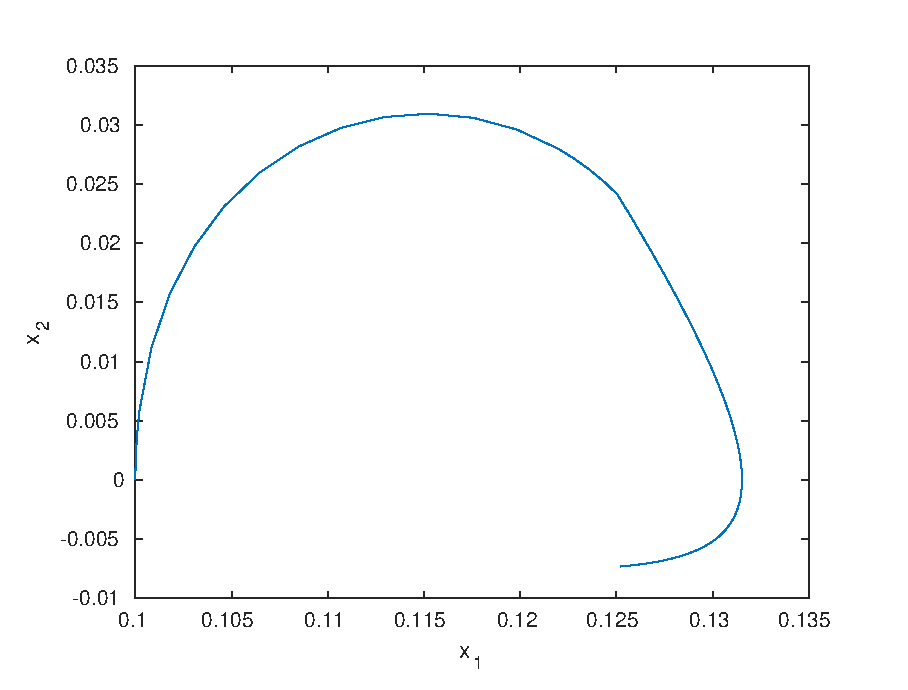
\includegraphics[width=0.7\textwidth]{x1x2.eps}\\
	{Рис. 1. }
\end{center}
	\begin{center}
	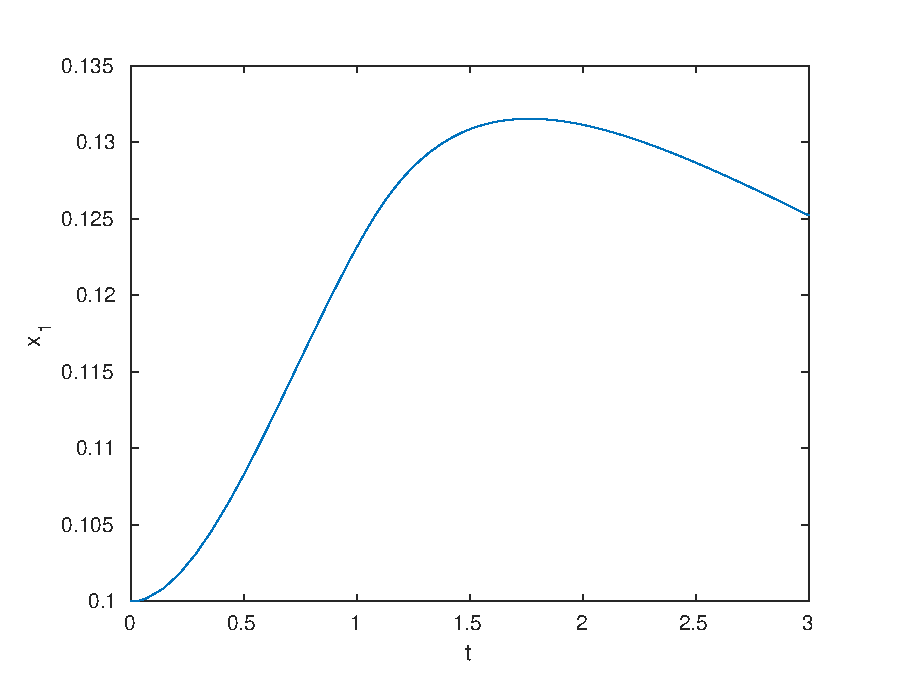
\includegraphics[width=0.7\textwidth]{x1t.eps}\\
	{Рис. 2. }
\end{center}
	\begin{center}
	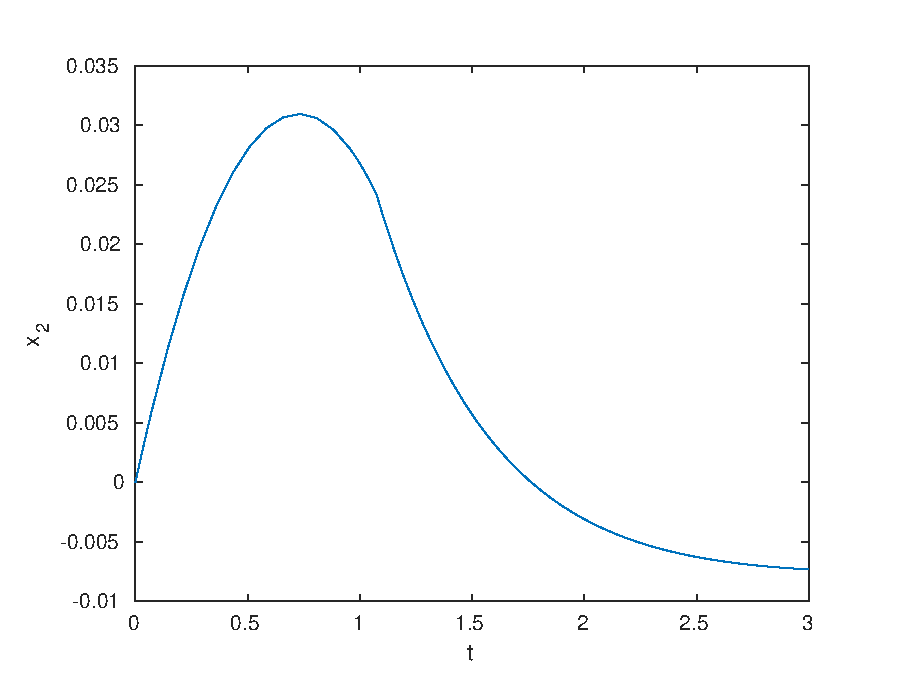
\includegraphics[width=0.7\textwidth]{x2t.eps}\\
	{Рис. 3. }
\end{center}
	\begin{center}
	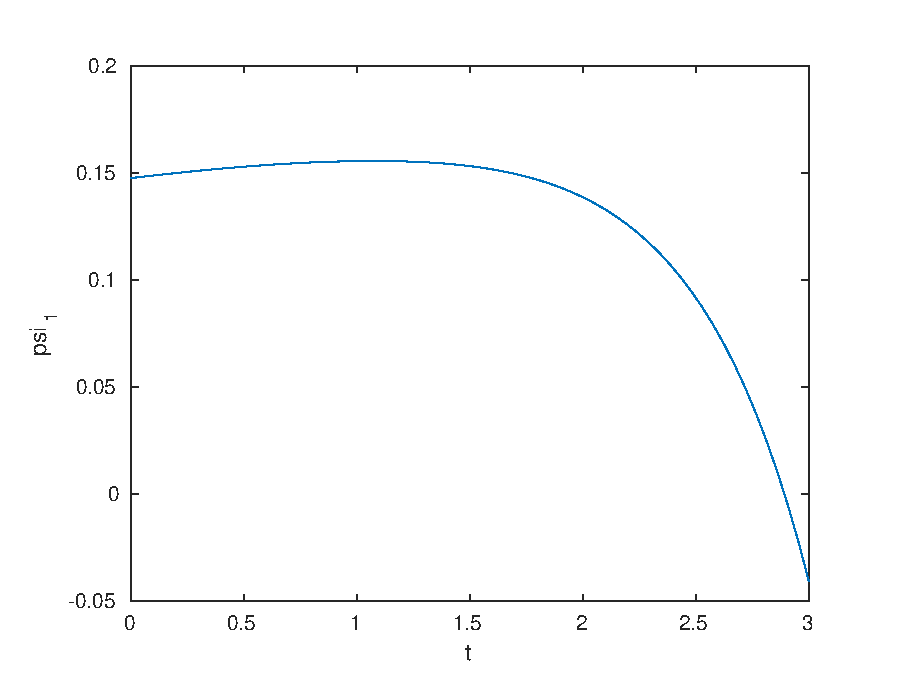
\includegraphics[width=0.7\textwidth]{psi1.eps}\\
	{Рис. 4. }
\end{center}
	\begin{center}
	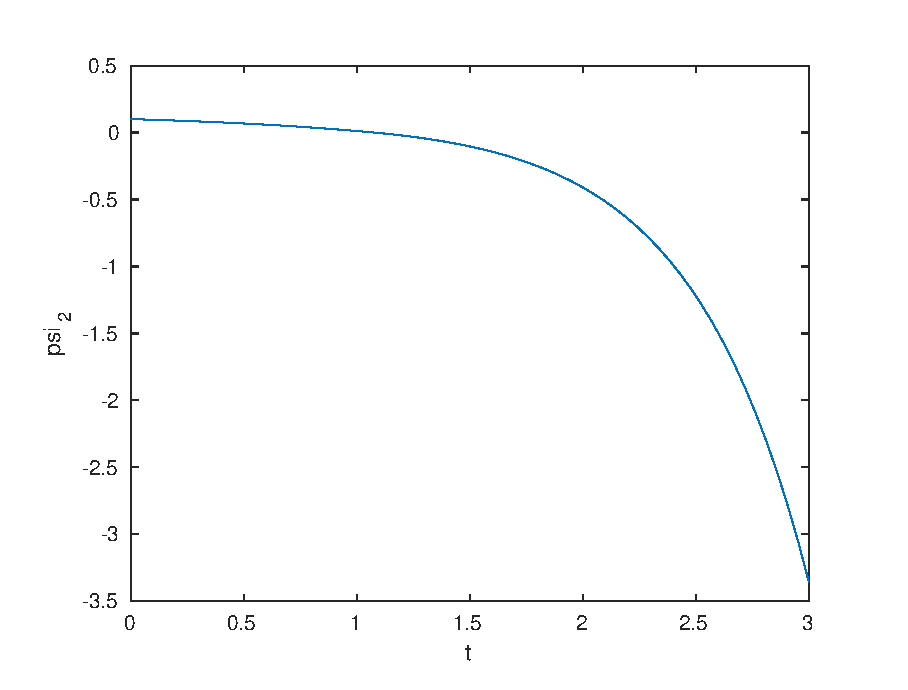
\includegraphics[width=0.7\textwidth]{psi2.eps}\\
	{Рис. 5. }
\end{center}
	\begin{center}
	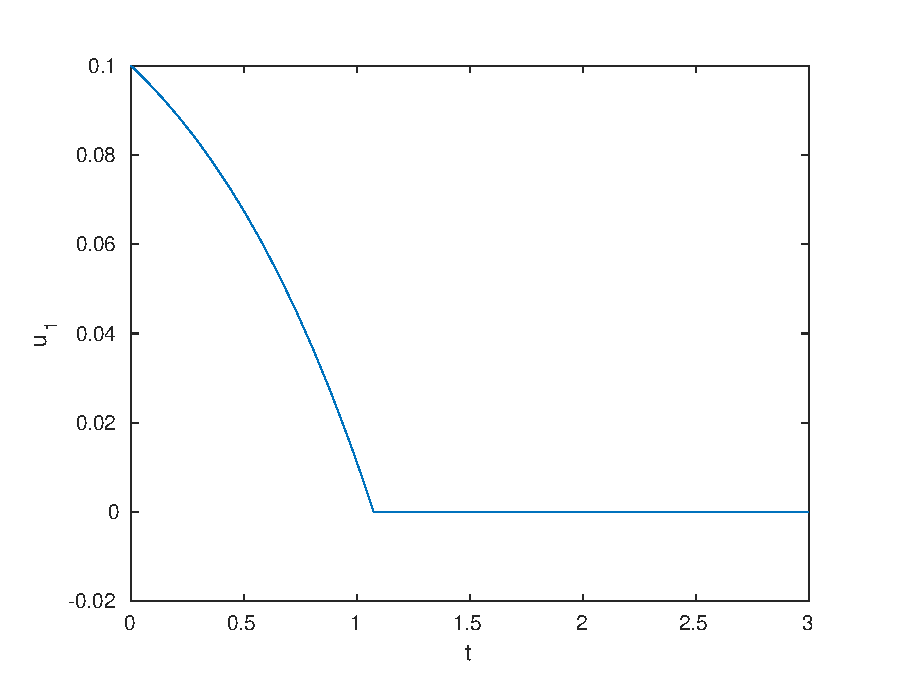
\includegraphics[width=0.7\textwidth]{u1t.eps}\\
	{Рис. 6. }
\end{center}
	\begin{center}
	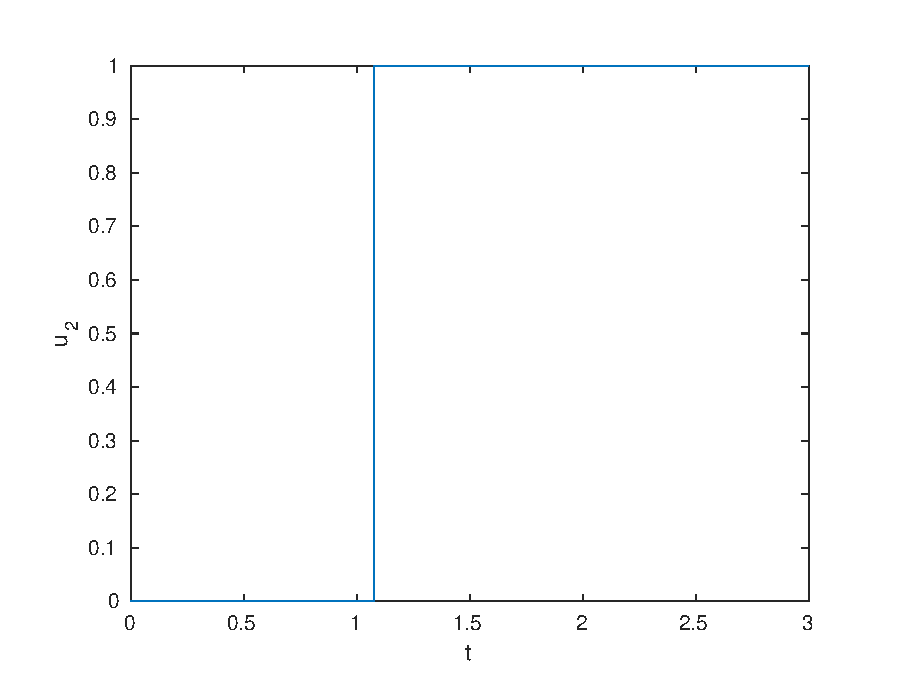
\includegraphics[width=0.7\textwidth]{u2t.eps}\\
	{Рис. 7. }
\end{center}
\newpage
{Решение задачи во втором случае. Параметры используются те же. $J(u) = 0.1987.$}
\begin{center}
	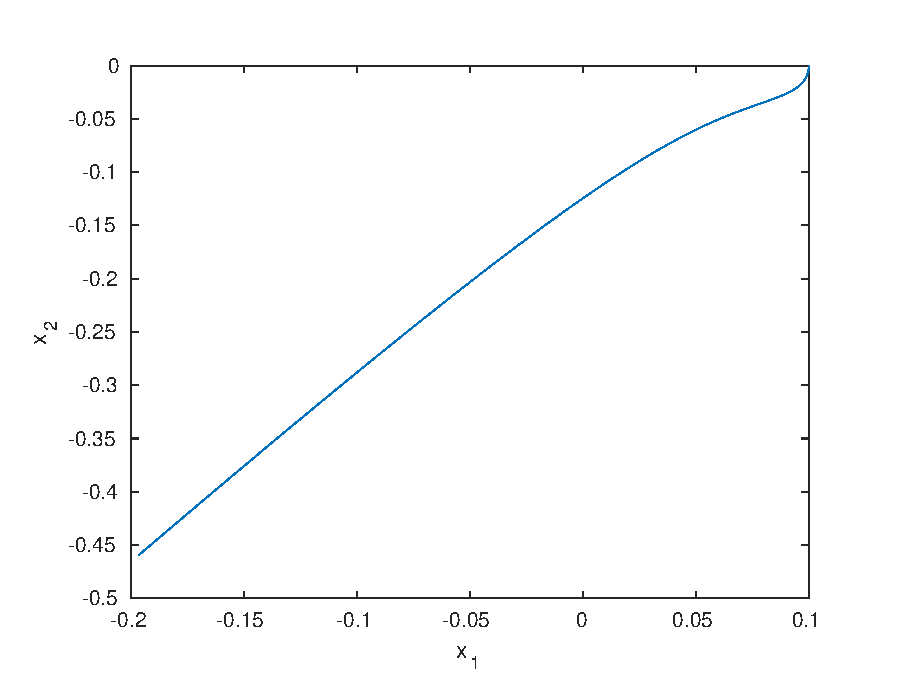
\includegraphics[width=0.7\textwidth]{x1x2_1.eps}\\
	{Рис. 8. }
\end{center}
\begin{center}
	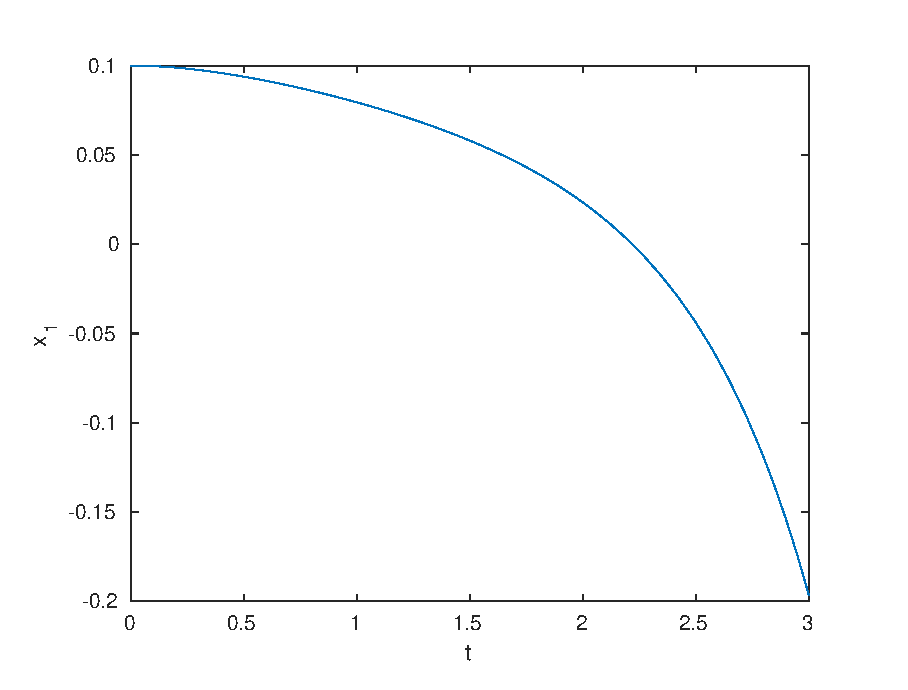
\includegraphics[width=0.7\textwidth]{x1t_1.eps}\\
	{Рис. 9. }
\end{center}
\begin{center}
	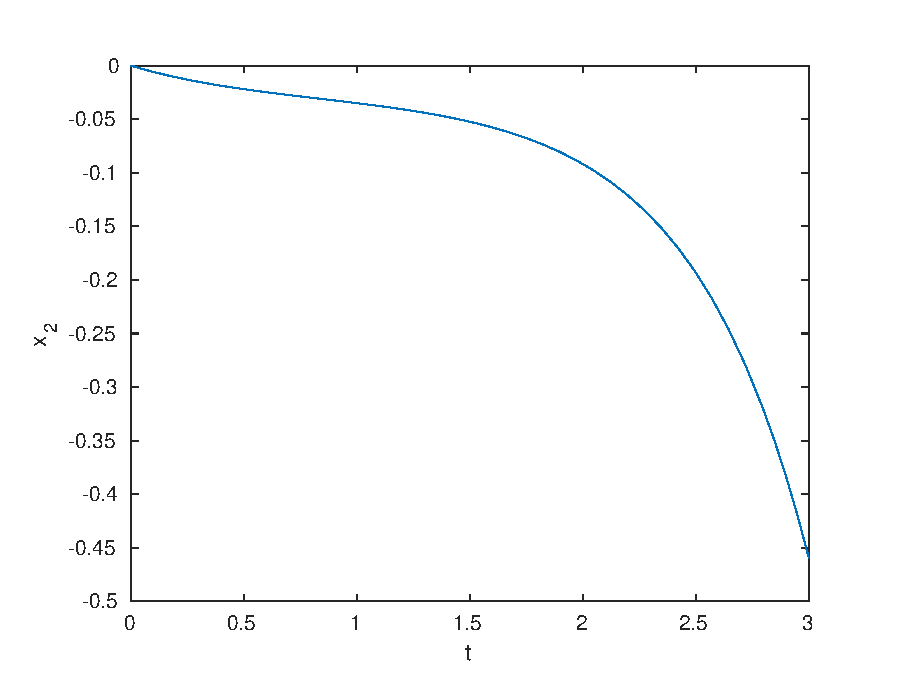
\includegraphics[width=0.7\textwidth]{x2t_1.eps}\\
	{Рис. 10. }
\end{center}
\begin{center}
	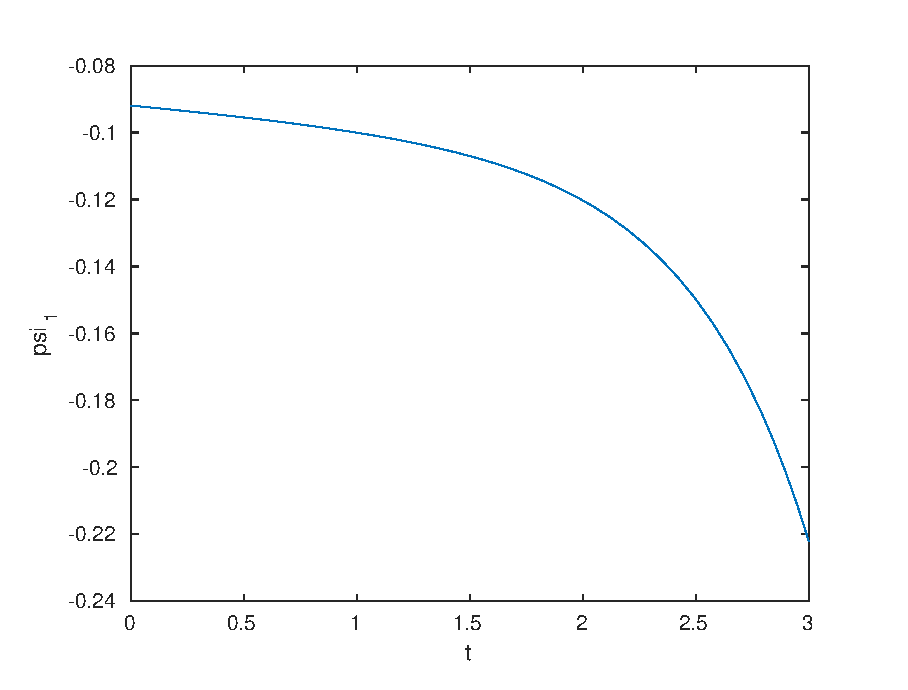
\includegraphics[width=0.7\textwidth]{psi1_1.eps}\\
	{Рис. 11. }
\end{center}
\begin{center}
	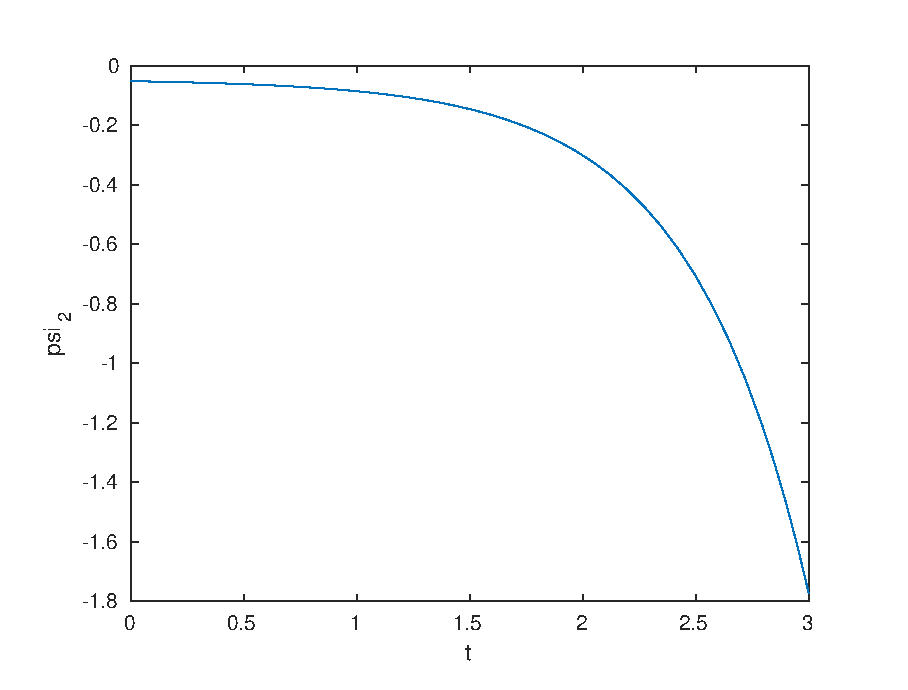
\includegraphics[width=0.7\textwidth]{psi2_1.eps}\\
	{Рис. 12. }
\end{center}
\begin{center}
	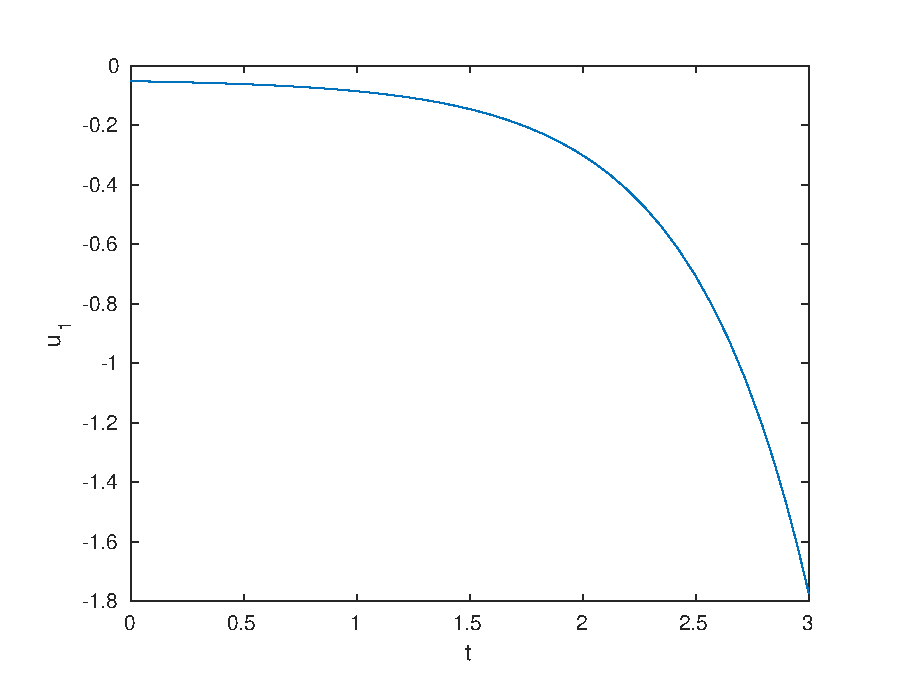
\includegraphics[width=0.7\textwidth]{u1t_1.eps}\\
	{Рис. 13. }
\end{center}
\begin{center}
	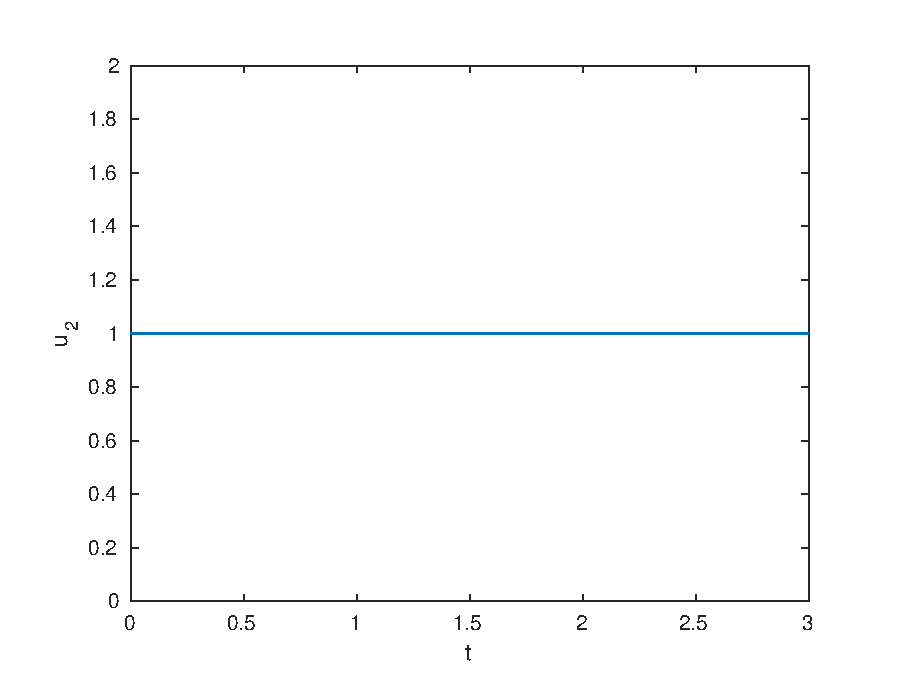
\includegraphics[width=0.7\textwidth]{u2t_1.eps}\\
	{Рис. 14. }
\end{center}
\newpage
\section{Список литературы}
{[1]Комаров Ю.А. Лекции и семинары по курсу Оптимальное управление. 2021.}
\end{document}